\documentclass{beamer}
\usetheme{JuanLesPins}
\usepackage{fontenc}

\usepackage[english]{babel}
\usepackage[latin1]{inputenc}
\usepackage{times}
\usepackage[T1]{fontenc}
\usepackage{fontenc}
\usepackage{amssymb}
%\usepackage{pgf,pgfarrows,pgfnodes,pgfautomata,pgfheaps}
\usepackage{amsmath,amssymb}
%\usepackage{tikz}
\usepackage{times}
\usepackage{colortbl}

\usebackgroundtemplate{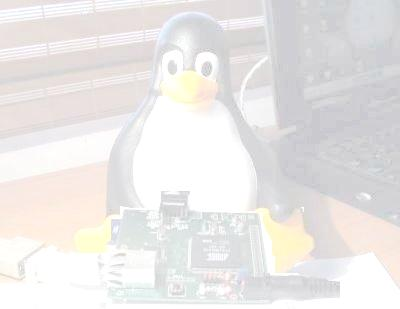
\includegraphics[width=\paperwidth, heigth=\paperheight]{../images/tux_ecb_at91.jpg}}

\title{El papel del Hardware copyleft en la Ense�anza de Sistemas Embebidos}
\author{Carlos Iv�n Camargo Bare�o}
\institute[Universidad Nacional de Colombia]{Universidad Nacional de Colombia\\
  Departamento de Ingenier�a El�ctrica y Electr�nica}

\pgfdeclareimage[height=.5cm]{logo}{../images/logo_unal}
\logo{\pgfuseimage{logo}}



\begin{document}

%----------------------------------------------------------------------INSERT TITLE-
\frame[c]{\titlepage}
\frame[c]{\tableofcontents}

%$$$$$$$$$$$$$$$$$$$$$$$$$$$$$$$$$$$$$$$$$$$$$$$$$$$$$$$$$$$$$$$$$$$$$$$$$$$$$$$$$$$
%----------------------------------------------------------------------Introducci�n-
\section{Sistemas Embebidos}
%$$$$$$$$$$$$$$$$$$$$$$$$$$$$$$$$$$$$$$$$$$$$$$$$$$$$$$$$$$$$$$$$$$$$$$$$$$$$$$$$$$$

\subsection[Embedded]{Aplicaciones}


\begin{frame}
  \frametitle{Sistemas Embebidos: Aplicaciones}
   \begin{center} 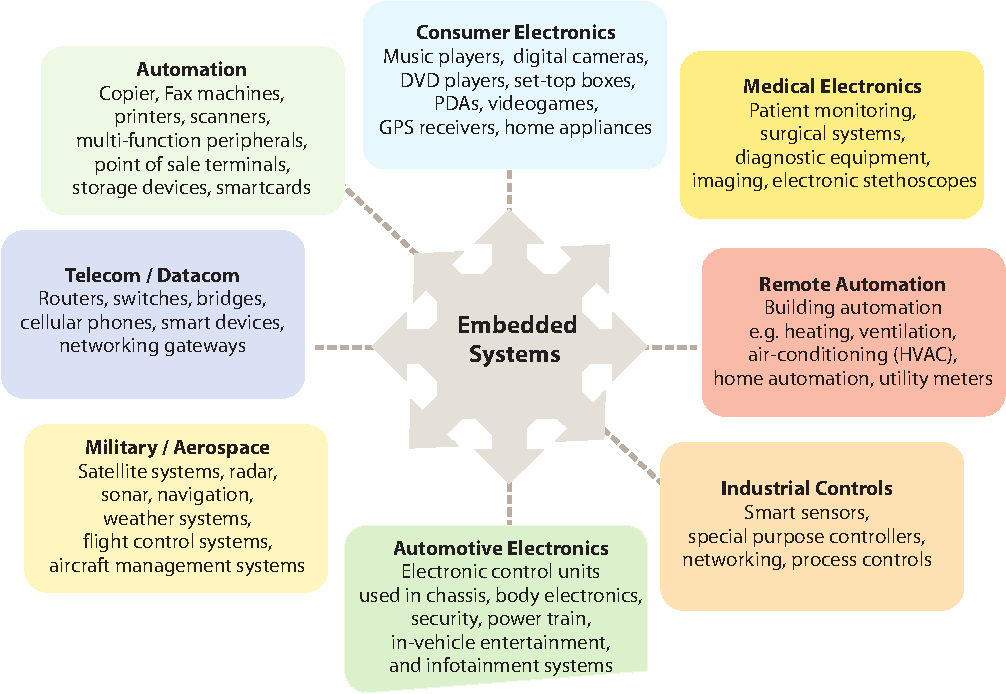
\includegraphics[scale=.55]{../images/Embedded_systems_applications.pdf}   \end{center}
\end{frame}


\subsection[Embedded]{Arquitectura}

\begin{frame}
  \frametitle{Sistemas Embebidos: Arquitectura}
   \begin{center} 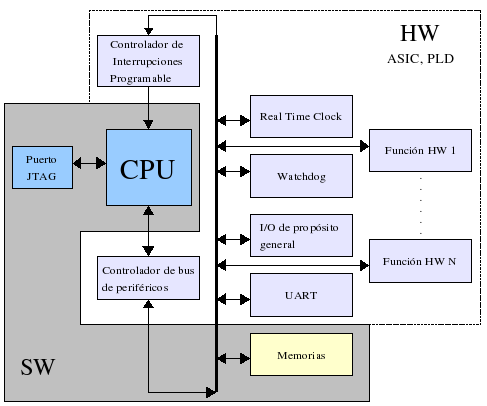
\includegraphics[scale=.5]{../images/ES_Architecture.png}   \end{center}
\end{frame}


\subsection[Embedded]{Conocimientos Necesarios}
\begin{frame}
  \frametitle{Sistemas Embebidos: Aplicaciones}
   \begin{center} 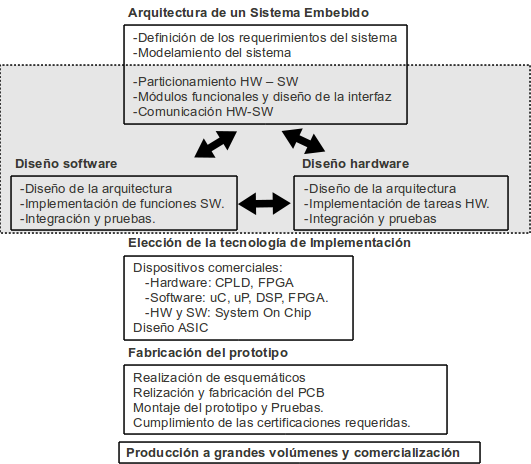
\includegraphics[scale=.51]{../images/ES_CDIO_flow.png}   \end{center}
\end{frame}



%$$$$$$$$$$$$$$$$$$$$$$$$$$$$$$$$$$$$$$$$$$$$$$$$$$$$$$$$$$$$$$$$$$$$$$$$$$$$$$$$$$$
%----------------------------------------------------------Metodolog�a de Ense�anza-
\section{Metodolog�a de Ense�anza}
%$$$$$$$$$$$$$$$$$$$$$$$$$$$$$$$$$$$$$$$$$$$$$$$$$$$$$$$$$$$$$$$$$$$$$$$$$$$$$$$$$$$

\begin{frame}
  \frametitle{Divisi�n implementada en la Universidad Nacional de Colombia}
 \begin{figure}[htpb]
   \begin{center} 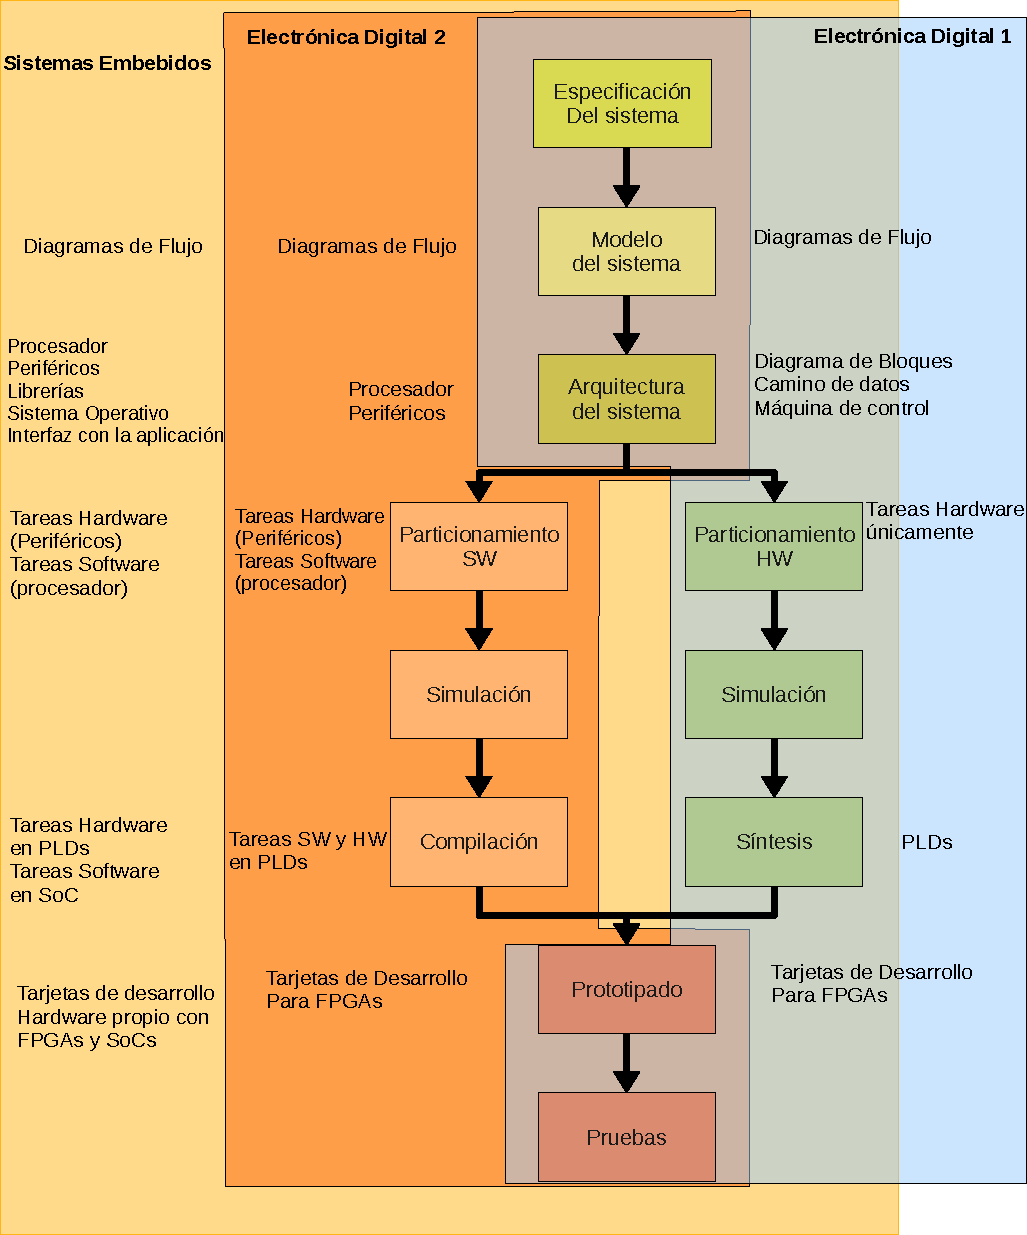
\includegraphics[scale=.33]{../images/habilidades_digitales.pdf}   \end{center}
 \end{figure}
\end{frame}

%$$$$$$$$$$$$$$$$$$$$$$$$$$$$$$$$$$$$$$$$$$$$$$$$$$$$$$$$$$$$$$$$$$$$$$$$$$$$$$$$$$$
%----------------------------------------------------------Metodolog�a de Ense�anza-
\section{Plataforma Copyleft Hardware SIE}
%$$$$$$$$$$$$$$$$$$$$$$$$$$$$$$$$$$$$$$$$$$$$$$$$$$$$$$$$$$$$$$$$$$$$$$$$$$$$$$$$$$$

\subsection{Especificaciones}

\begin{frame}
  \frametitle{SIE: Especificaciones}
 \begin{figure}[htpb]
   \begin{center} 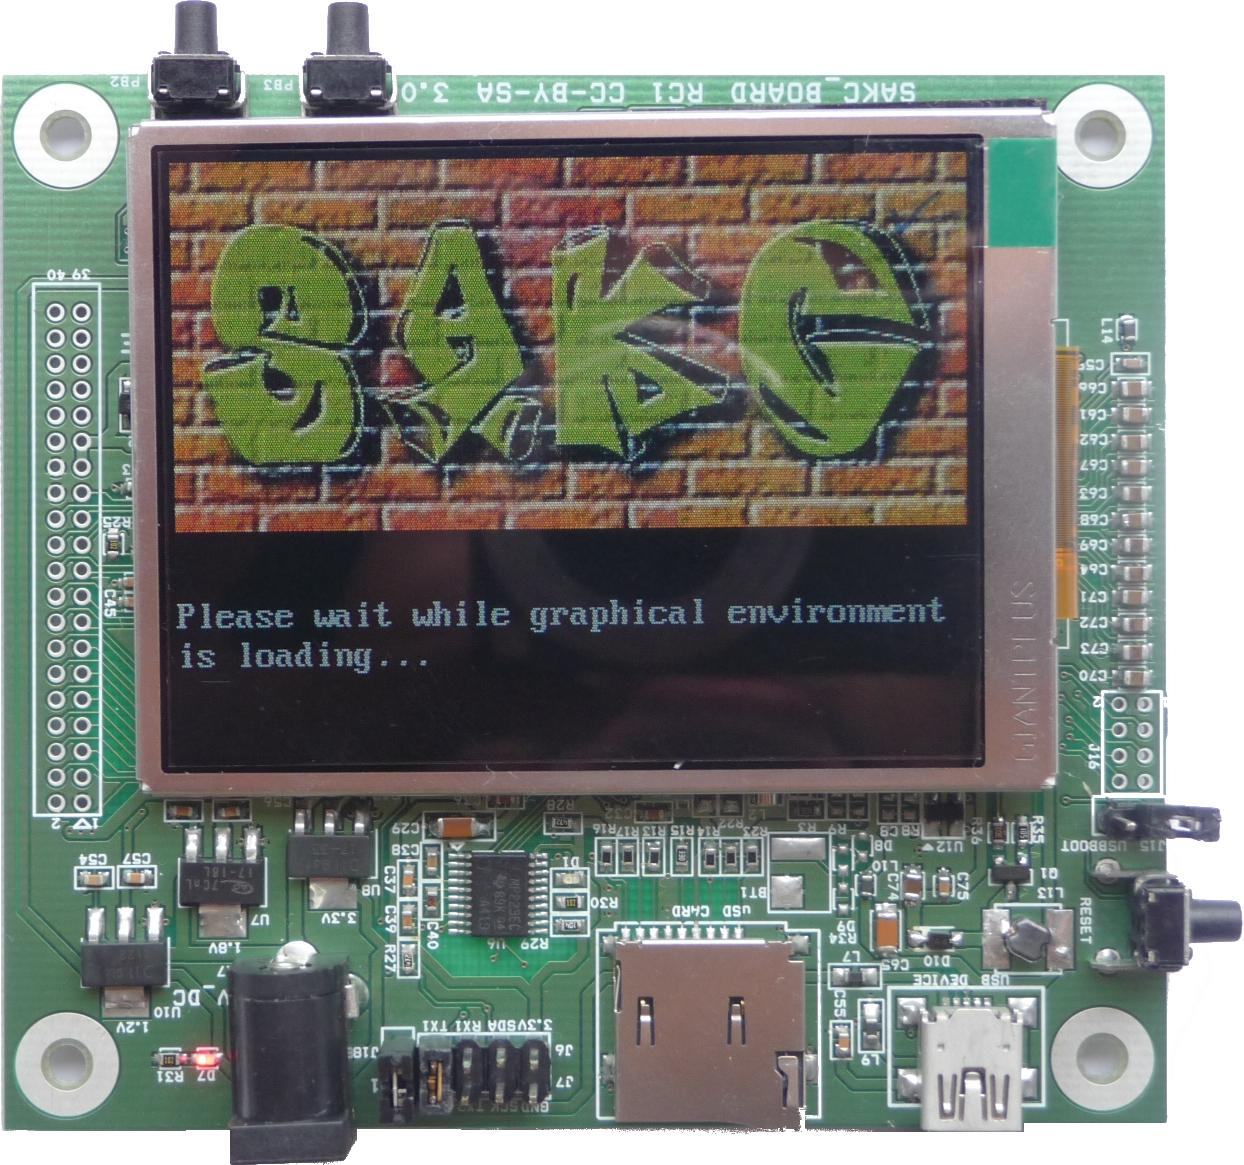
\includegraphics[scale=.5]{../images/SIE.jpg}   \end{center}
 \end{figure}
\end{frame}

\subsection{Diagrama de Bloques}

\begin{frame}
  \frametitle{SIE: Diagrama de Bloques}
 \begin{figure}[htpb]
   \begin{center} 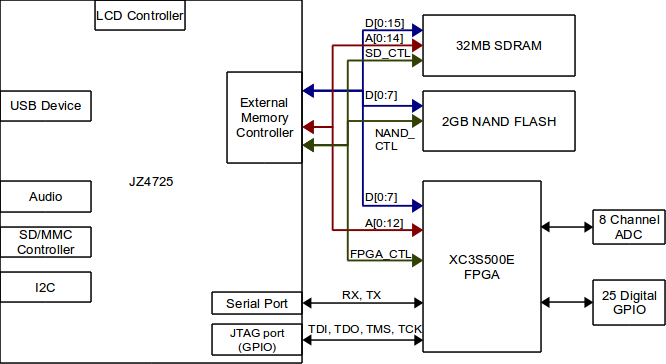
\includegraphics[scale=.5]{../images/SIE_block_diagram.png}   \end{center}
 \end{figure}
\end{frame}

\subsection{SIE: Plataforma hardware copyleft }
 
 \begin{frame}

  \frametitle{SIE: Plataforma hardware copyleft}

     \begin{block}{ }
      \begin{itemize}
       \item Acceso a los archivos de dise�o realizados en herramientas abiertas (kicad en este caso)
       \item Posibilidad de hacer cambios f�sicos y funcionales.
       \item Acceso a notas de aplicaci�n, dise�os de referencia.
       \item Acceso al software b�sico: \textit{bootloader} \textit{kernel} \textit{sistema de archivos}
       \item Soporte a trav�s de listas de discusi�n.
       \item Acceso a los fabricantes de las tarjetas.
      \end{itemize}
     \end{block}

    \begin{alertblock}{}
      Todo esto puede descargarse de: http://wiki.linuxencaja.net/wiki/GIT
    \end{alertblock}

 \end{frame}

 \begin{frame}


     \begin{alertblock}{Licencia: Creative Commons BY - SA}
      \textbf{BY} Permite distribuir, modificar y construir sobre su trabajo, incluso con fines comerciales, siempre y cuando se de cr�dito a la creaci�n original.                                   \\
      \textbf{BY - SA}: Todo trabajo derivado debe tener la misma licencia.
     \end{alertblock}


 
 \end{frame}



%$$$$$$$$$$$$$$$$$$$$$$$$$$$$$$$$$$$$$$$$$$$$$$$$$$$$$$$$$$$$$$$$$$$$$$$$$$$$$$$$$$$
%----------------------------------------------------------Metodolog�a de Ense�anza-
\section{SIE en la Ense�anza de Dise�o Digital}
%$$$$$$$$$$$$$$$$$$$$$$$$$$$$$$$$$$$$$$$$$$$$$$$$$$$$$$$$$$$$$$$$$$$$$$$$$$$$$$$$$$$

\begin{frame}
  \frametitle{SIE en el curso b�sico de digitales}
   \begin{center} 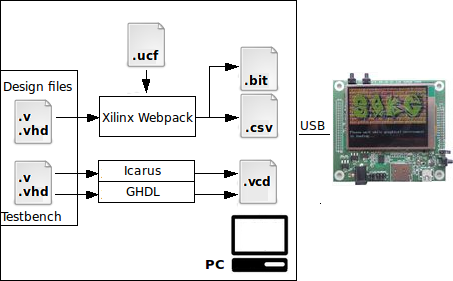
\includegraphics[scale=.75]{../images/HW_design_flow.png}   \end{center}
\end{frame}

\begin{frame}
 \begin{figure}[htpb]
  \frametitle{SIE en el curso b�sico de Arquitectura de Computadores}
   \begin{center} 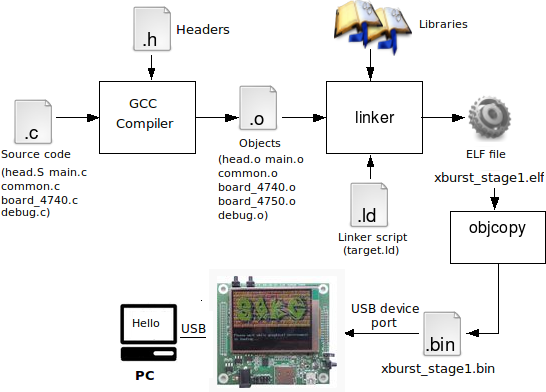
\includegraphics[scale=.55]{../images/SW_design_flow.png}   \end{center}
 \end{figure}
\end{frame}


\begin{frame}
  \frametitle{Interfaz HW/SW de SIE}
   \begin{center} 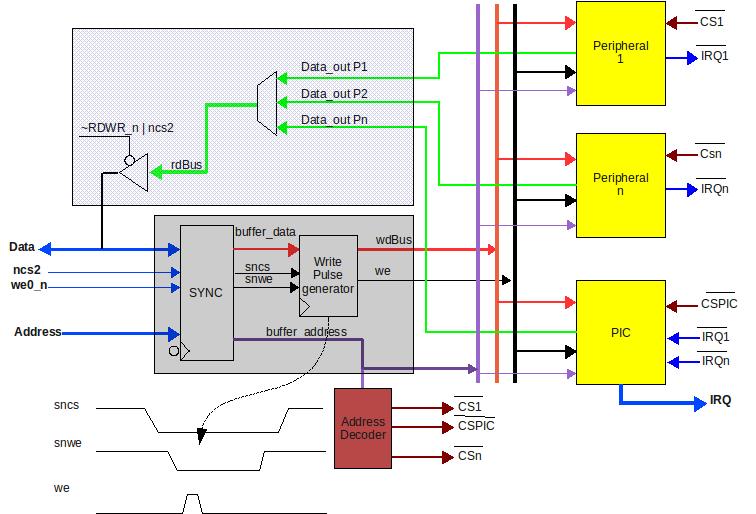
\includegraphics[scale=.45]{../images/Sw_hw_fpga_arch.png}   \end{center}
\end{frame}


\begin{frame}
  \frametitle{SIE en el curso Sistemas Embebidos}
   \begin{center} 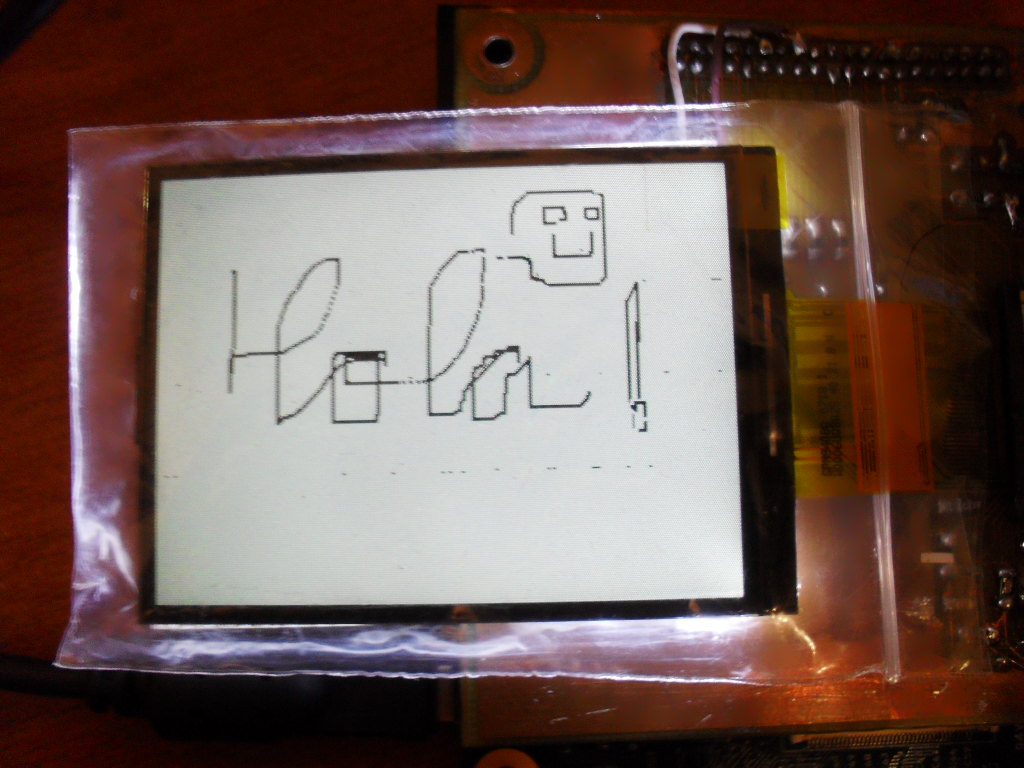
\includegraphics[scale=.15]{../images/Academic_Paint.JPG}   
                  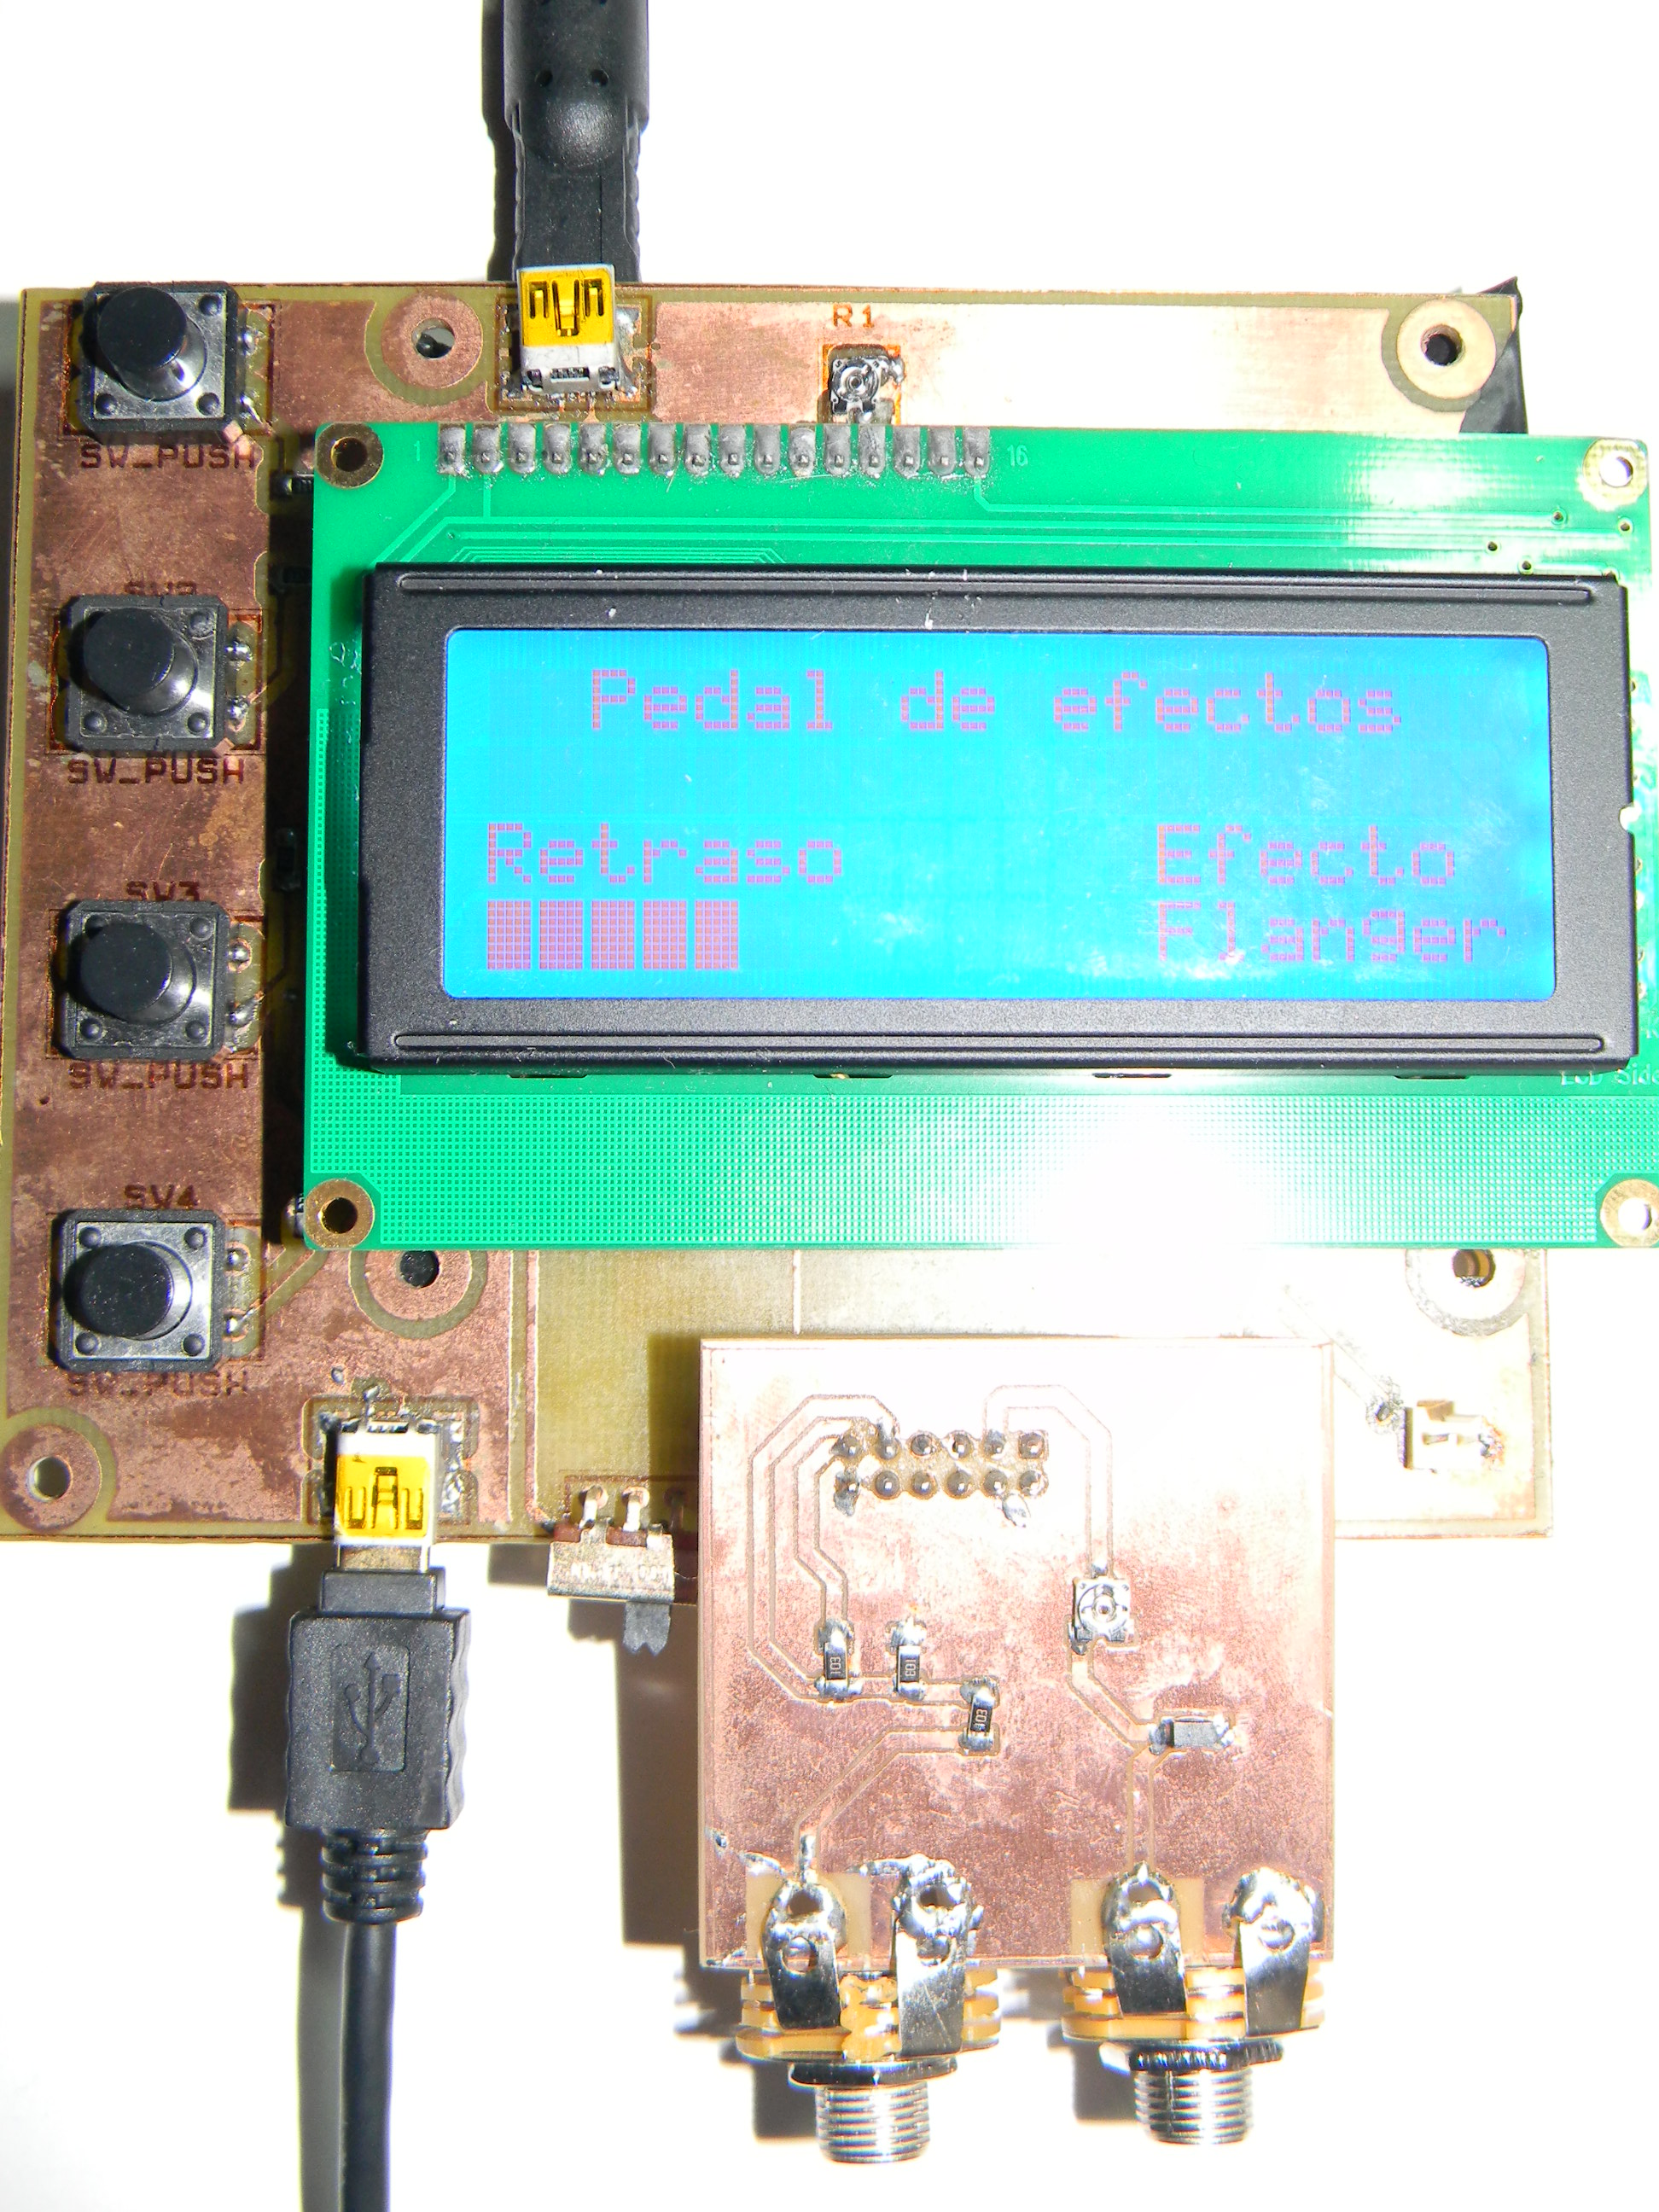
\includegraphics[scale=.05]{../images/Academic_Pedal.JPG}   \\
                  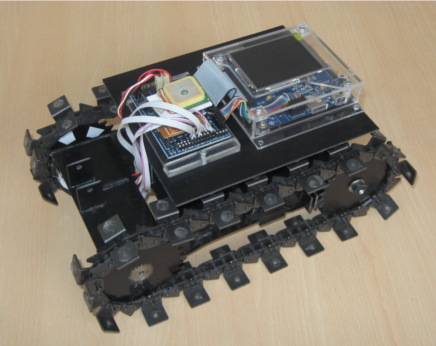
\includegraphics[scale=.3]{../images/Academic_Siebot.png}   
                  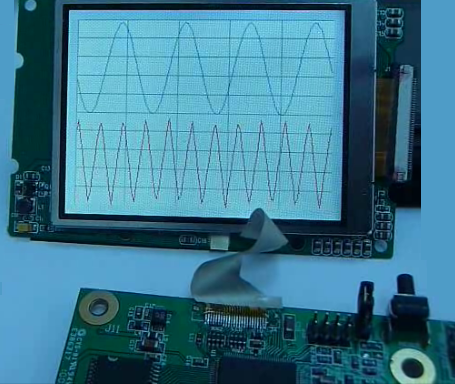
\includegraphics[scale=.35]{../images/Academic_Scop.png}   
   \end{center} 
\end{frame}


\begin{frame}
  \frametitle{Opini�n de los Estudiantes \footnote{Encuesta realizada a 60 estudiantes de los cursos de \textit{Arquitectura de Compuatdores} y \textit{Sistemas Embebidos}}
}
       \begin{block}{}
         \begin{itemize}
          \item Encuentran la metodolog�a adecuada para generar habilidades necesarias para el desarrollo de aplicaciones comerciales
          \item Se proporcionan las herramientas necesarias para lograr el objetivo final.
          \item Son conscientes de que se busca que ellos generen productos novedosos y de esta forma generar empleo.
          \item Se muestra que los estudiantes no tienen ning�n problema en utilizar herramientas licenciadas de forma ilegal.
          \item Prefieren el uso de las herramientas libres aunque su utilizaci�n sea mas compleja.
         \end{itemize}
       \end{block}
\end{frame}

\begin{frame}
  \frametitle{Conclusiones}
       \begin{alertblock}{}
         \begin{itemize}
          \item El hardware copyleft es una herramienta poderosa para la creaci�n de habilidades necesarias para concebir, dise�ar, implementar y operar sistemas digitales
          \item Las actividades propuestas en las tres asignaturas del �rea tienen como objetivo generar en el estudiante las habilidades necesarias que le permitan dise�ar sistemas digitales con grado de complejidad creciente, hasta llegar a un sistema que puede ser comercializable y satisface una necesidad de una determinada comunida
          \item La utilizaci�n de herramientas de bajo nivel permite que el estudiante conozca y controle los diferentes pasos de la metodolog�a de dise�o y sea capaz de ajustarlas para diferentes situaciones, esto hace que se adquiera un conocimiento sobre la tecnolog�a sin crear dependencia
         \end{itemize}
       \end{alertblock} 
\end{frame}



 
 \begin{frame}
   \begin{center}
\includegraphics[scale=.15]{../images/gracias}
   \newline
   \huge{�Gracias!}
   \end{center}
 \end{frame}

\end{document}
